%%%%%%%%%%%%%%%%%%%%%%%%%%%%%%%%%%%%%%%%%%%%%%%%%%%
%
%  New template code for TAMU Theses and Dissertations starting Fall 2016.
%
%
%  Original Author: Sean Zachary Roberson
%  This version adapted for URS by Parasol lab.
%  Adapted from version 3.16.10, which was last updated on 9/29/2016.
%  URS adaptation last updated 1/9/2017.
%
%%%%%%%%%%%%%%%%%%%%%%%%%%%%%%%%%%%%%%%%%%%%%%%%%%%
%%%%%%%%%%%%%%%%%%%%%%%%%%%%%%%%%%%%%%%%%%%%%%%%%%%%%%%%%%%%%%%%%%%%%%
%%                           CONCLUSION
%%%%%%%%%%%%%%%%%%%%%%%%%%%%%%%%%%%%%%%%%%%%%%%%%%%%%%%%%%%%%%%%%%%%%

\chapter{CONCLUSION}

\section{Results}

Images of the application and textbook?

\begin{figure}[ht]
    \centering
    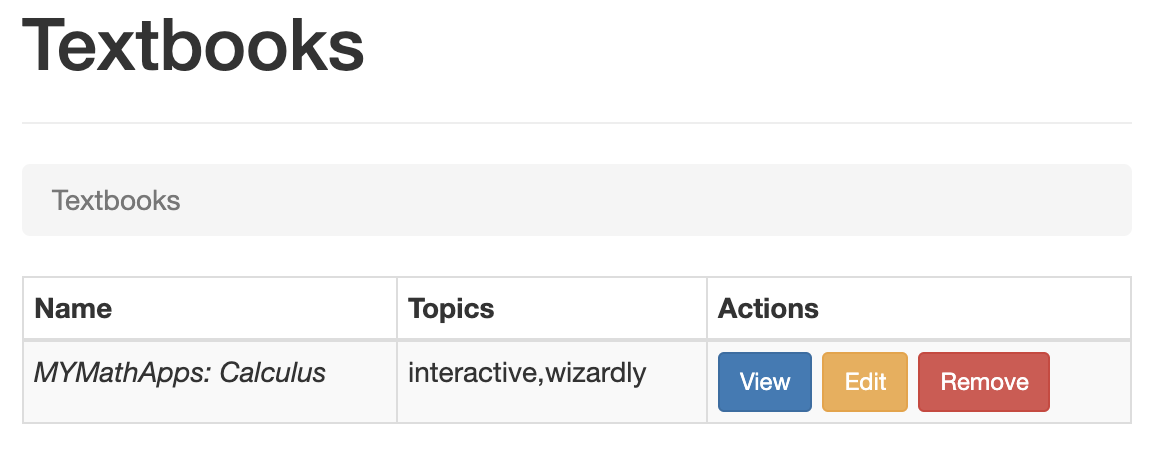
\includegraphics[scale=0.75]{textbooks.png}
    \caption[Unrelated topics.]{Unrelated topics. Can have any number of parents and children but do not relate to one another.}
        
    \label{fig:textbooks}
\end{figure}

\begin{figure}[ht]
    \centering
    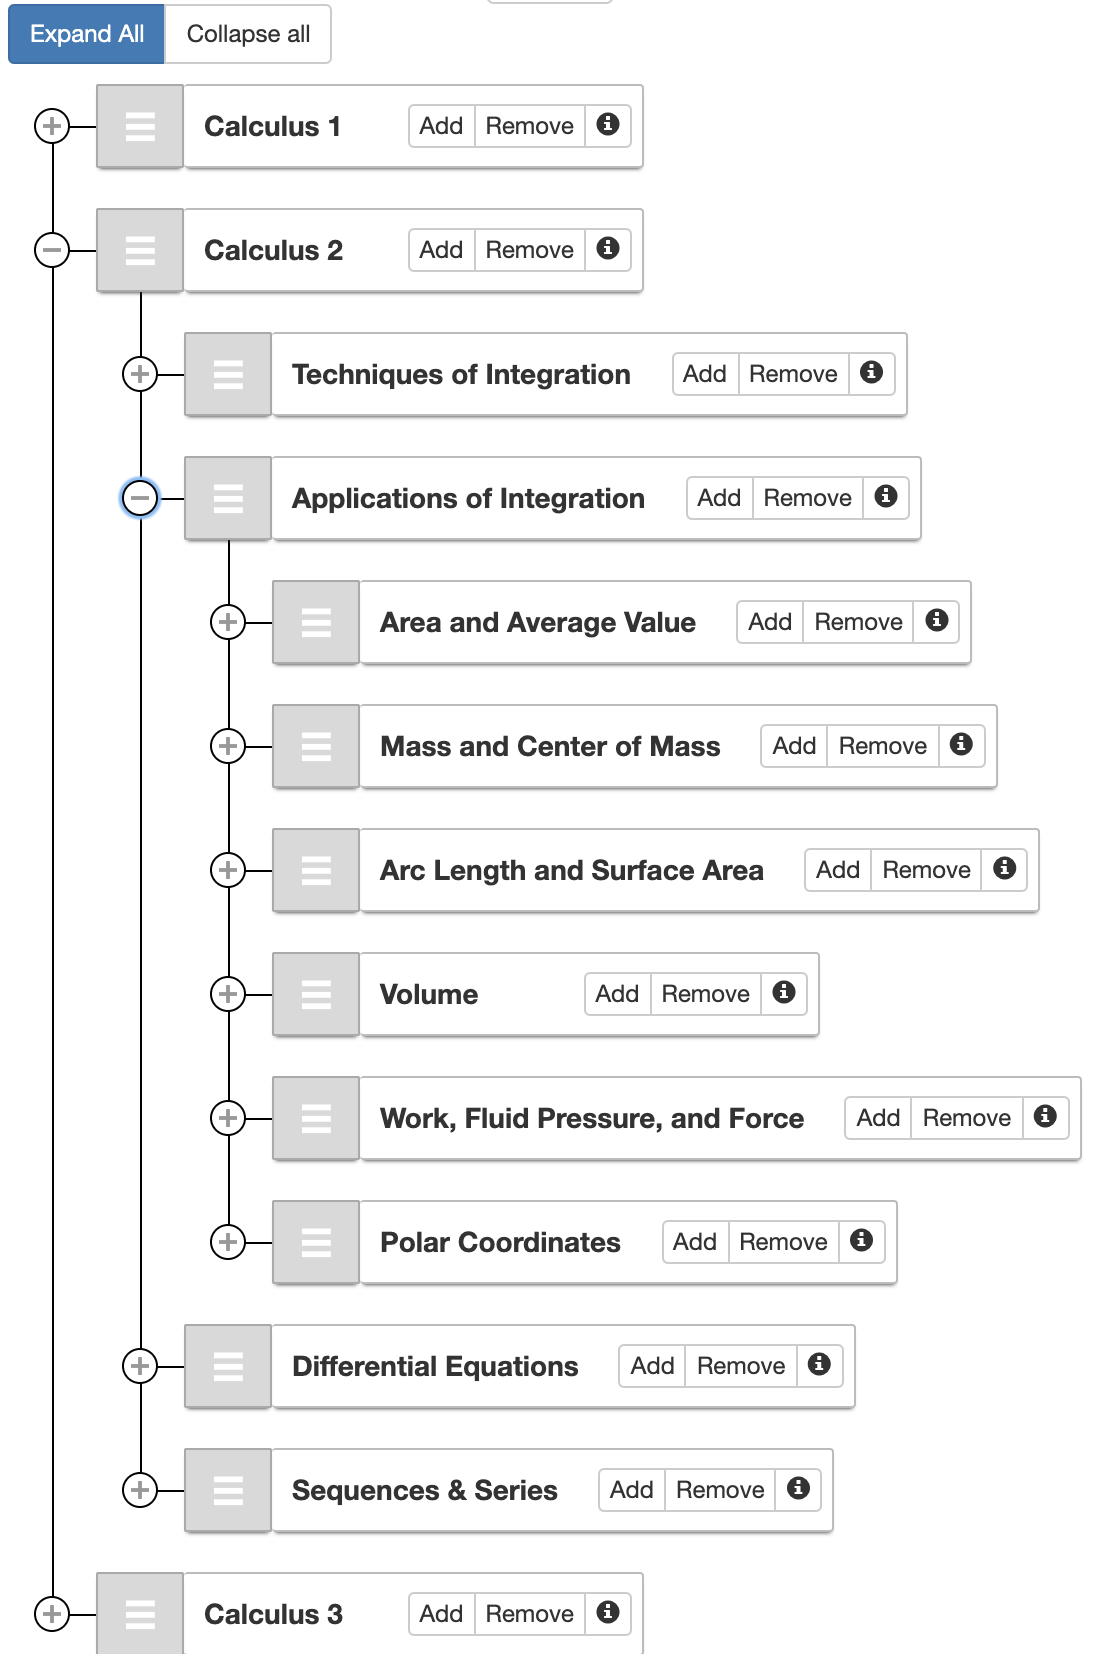
\includegraphics[scale=0.5]{nestedChapters.png}
    \caption[Unrelated topics.]{Unrelated topics. Can have any number of parents and children but do not relate to one another.}
        
    \label{fig:nestedChapters}
\end{figure}

\begin{figure}[ht]
    \centering
    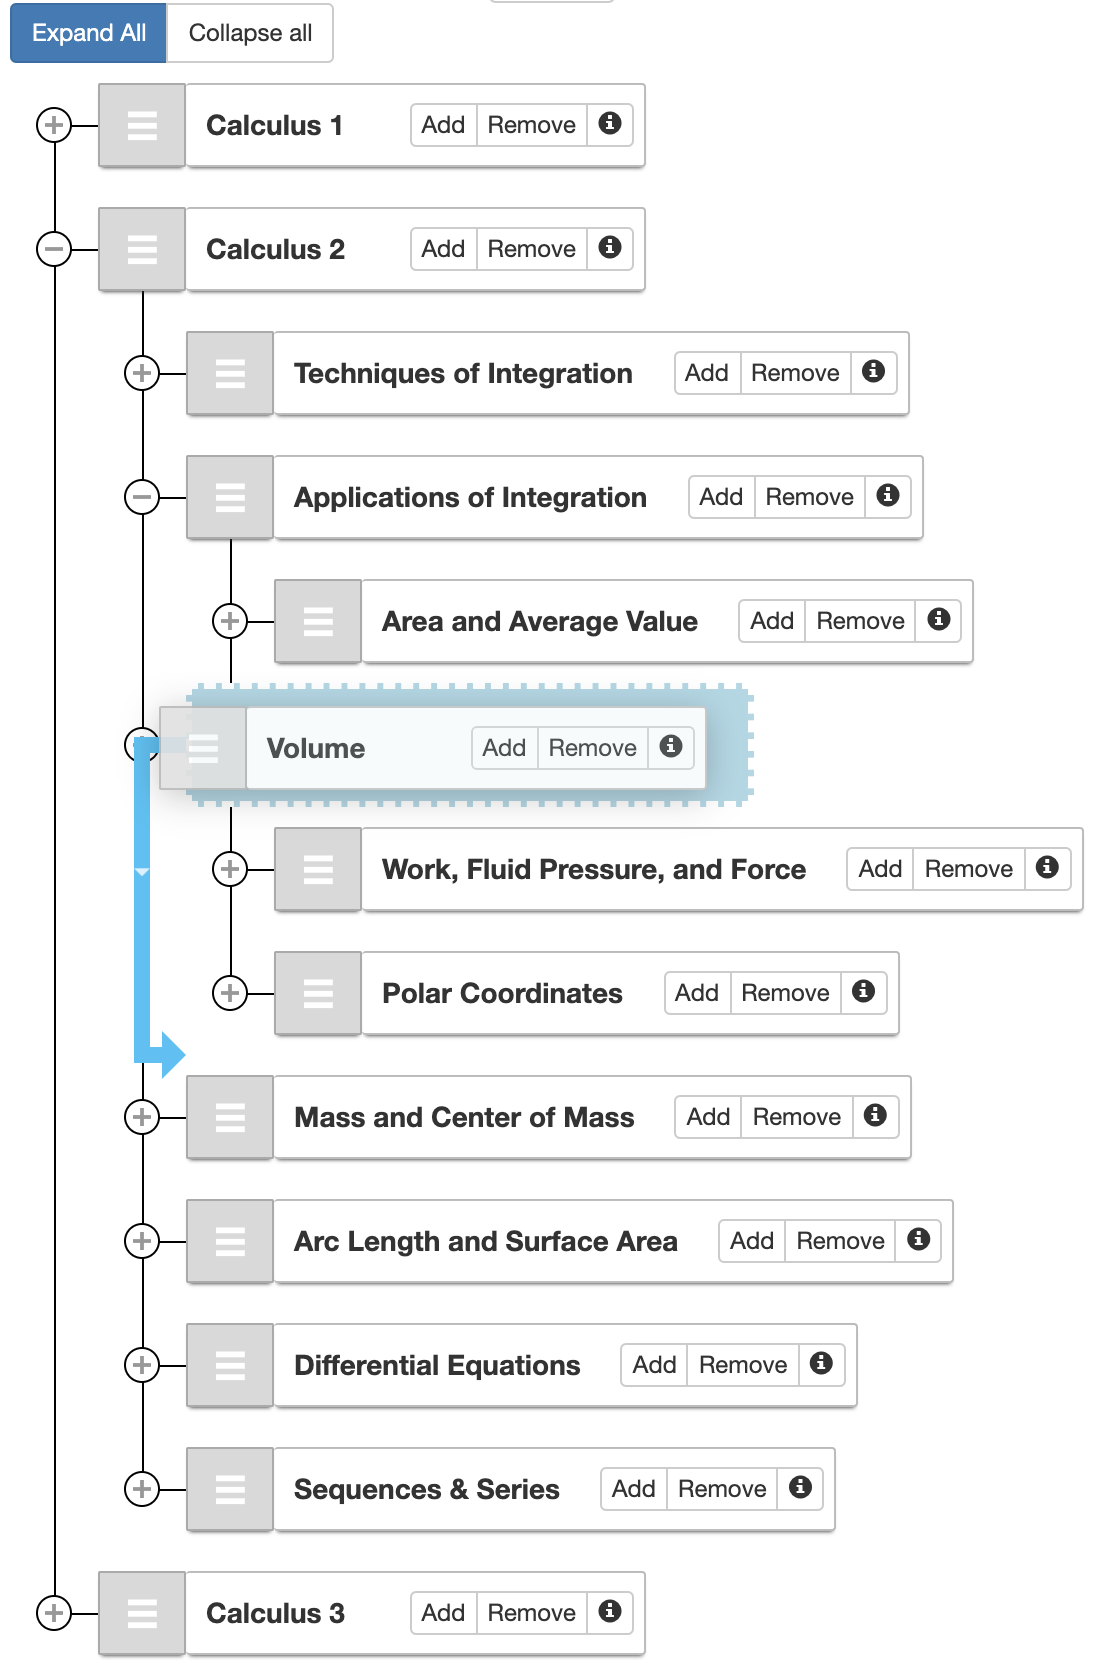
\includegraphics[scale=0.5]{chaptersMoving.png}
    \caption[Unrelated topics.]{Unrelated topics. Can have any number of parents and children but do not relate to one another.}
        
    \label{fig:chaptersMoving}
\end{figure}

\section{Challenges}

Time, takin 23 credit hrs ect\dots?
Tweaking existing build process of textbook for integration.

\section{Broader Impact}

Allow other authors to utilize this design + implementation?

\section{Future Plans}

Get this functional for entire MYMACalc book
